\taskpic{ Две материальные точки 1 и 2 и точечный источник света $S$
  совершают равномерное прямолинейное движение по горизонтальной
  плоскости. Тени от материальных точек 1 и 2 движутся со скоростями
  $u$ вдоль вертикальных стенок, которые перпендикулярны друг
  другу. Скорости материальных точек равны $v=2u/\sqrt{3}$ и
  направлены под углом $\alpha=30^{\circ}$ к соответствующим стенкам
  (см. рисунок).  Чему равна и куда направлена скорость источника $S$? }
{
  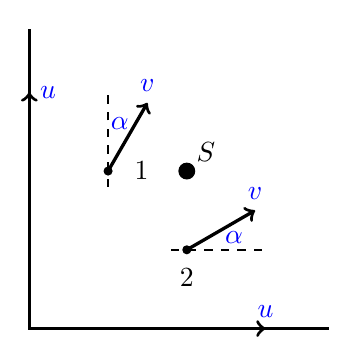
\begin{tikzpicture}
    \draw[very thick] (3.8,0) -- (0,0) -- (0,3.8);
    \draw[very thick,->] (0,0) -- (3,0) node[blue,above] {$u$};
    \draw[very thick,->] (0,0) -- (0,3) node[blue,right] {$u$};
    \draw[very thick,->] (1,2) node[right=0.2cm] {1} -- ++(60:1cm)
    node[blue,above] {$v$}; 
    \draw[very thick,->] (2,1) node[below=0.1cm] {2} -- ++(30:1cm)
    node[blue,above] {$v$};
    \draw[fill=black] (2,2) circle (0.1cm) node[above right] {$S$};
    \draw[dashed,thick] (1.8,1) -- (3,1);
    \draw[dashed,thick] (1,1.8) -- (1,3);
    \draw (1.15,2.6) node[blue] {$\alpha$};
    \draw (2.6,1.15) node[blue] {$\alpha$};
    \draw[fill=black] (1,2) circle (0.05cm);
    \draw[fill=black] (2,1) circle (0.05cm);
  \end{tikzpicture}
}
% Москва, город-2001, 9 класс